Since $u(x, t) \to 0$ as $x \to +\infty$ and $u(x, t) \to 1$ as $x \to -\infty$, we can approximate the traveling wave
given in (i) on $[-L, L]$, where $L$ is large enough that the wave front does not reach the boundary $x = L$ by imposing
the boundary conditions

$$
u(-L, t) = 1 \quad \text{and} \quad u(L, t) = 0
$$

with initial value $u(x, 0)$. Design and implement a Chebyshev collocation method to approximate the solution to the
PDE and study the convergence of the approximate solution as $L \to \infty$.

\begin{solution}
    We begin by introducing the mapping $\xi : [-L, L] \to [-1, 1]$ defined by $\xi(x) = \frac{x}{L}$ 
    (and $\xi^{-1}(v) = Lx$). We define $u(x, t) = v(\xi, t)$; by the chain rule our PDE becomes the following
    boundary value problem:

    $$
    v_t = \frac{1}{L^2} v_{\xi\xi} + v(1 - v),  \quad v(-1, t) = 1, \quad v(1, t) = 0.
    $$

    upon which we impose the initial condition

    $$
    v_0 = u(L x, 0) = \left[ 1 + e^{\frac{Lx}{\sqrt{6}}} \right]^{-2}.
    $$

    Since we now have a BVP in $v(\xi, t)$ defined on $\xi = [-1, 1]$, we can use Chebyshev collocation in space to 
    approximate the solution. We utilize a forward Euler method in time to approximate the time derivative and implement
    this method in \texttt{problem\_2ii.m}. 

    \begin{figure}[h]
        \centering
        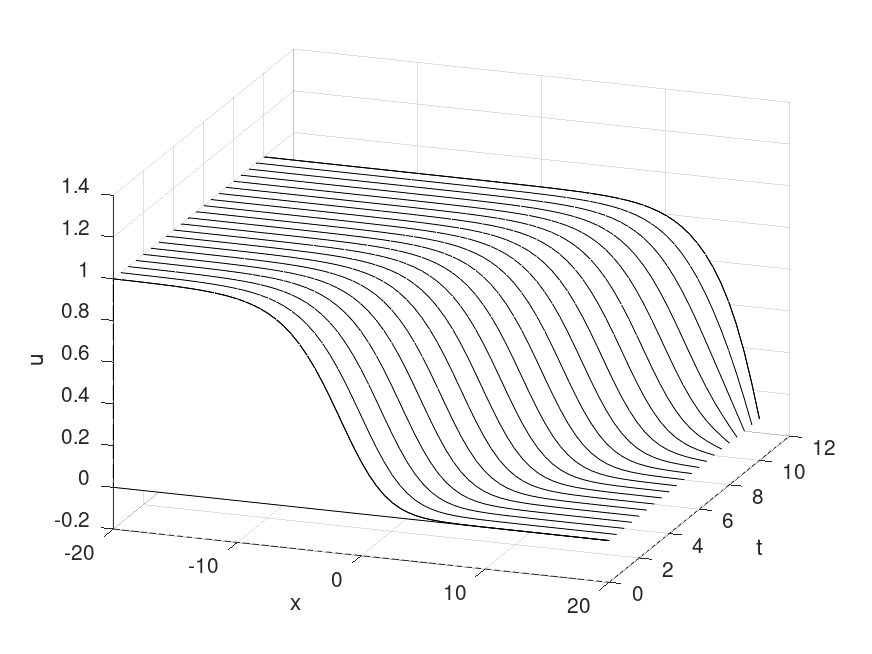
\includegraphics[width=0.70\textwidth]{problem_2ii_L20.png}
        \caption{Solution to Fisher PDE BVP on $L = [-20, 20]$.}
        \label{fig:problem_2ii_L20}
    \end{figure} 
    
    In Figure (\ref{fig:problem_2ii_L20}), we observe good convergence toward 
    the desired "front wave" solution with little numerical instability at $L = 20$. Conversely, we see in Figure 
    (\ref{fig:problem2ii_L30_L60}) that numerical instabilities are introduced at $L = 30,40,60$, but the method still 
    demonstrates general convergence to the expected solution.

    \begin{figure*}[h]
        \centering
        \begin{subfigure}[b]{0.49\textwidth}
            \centering
            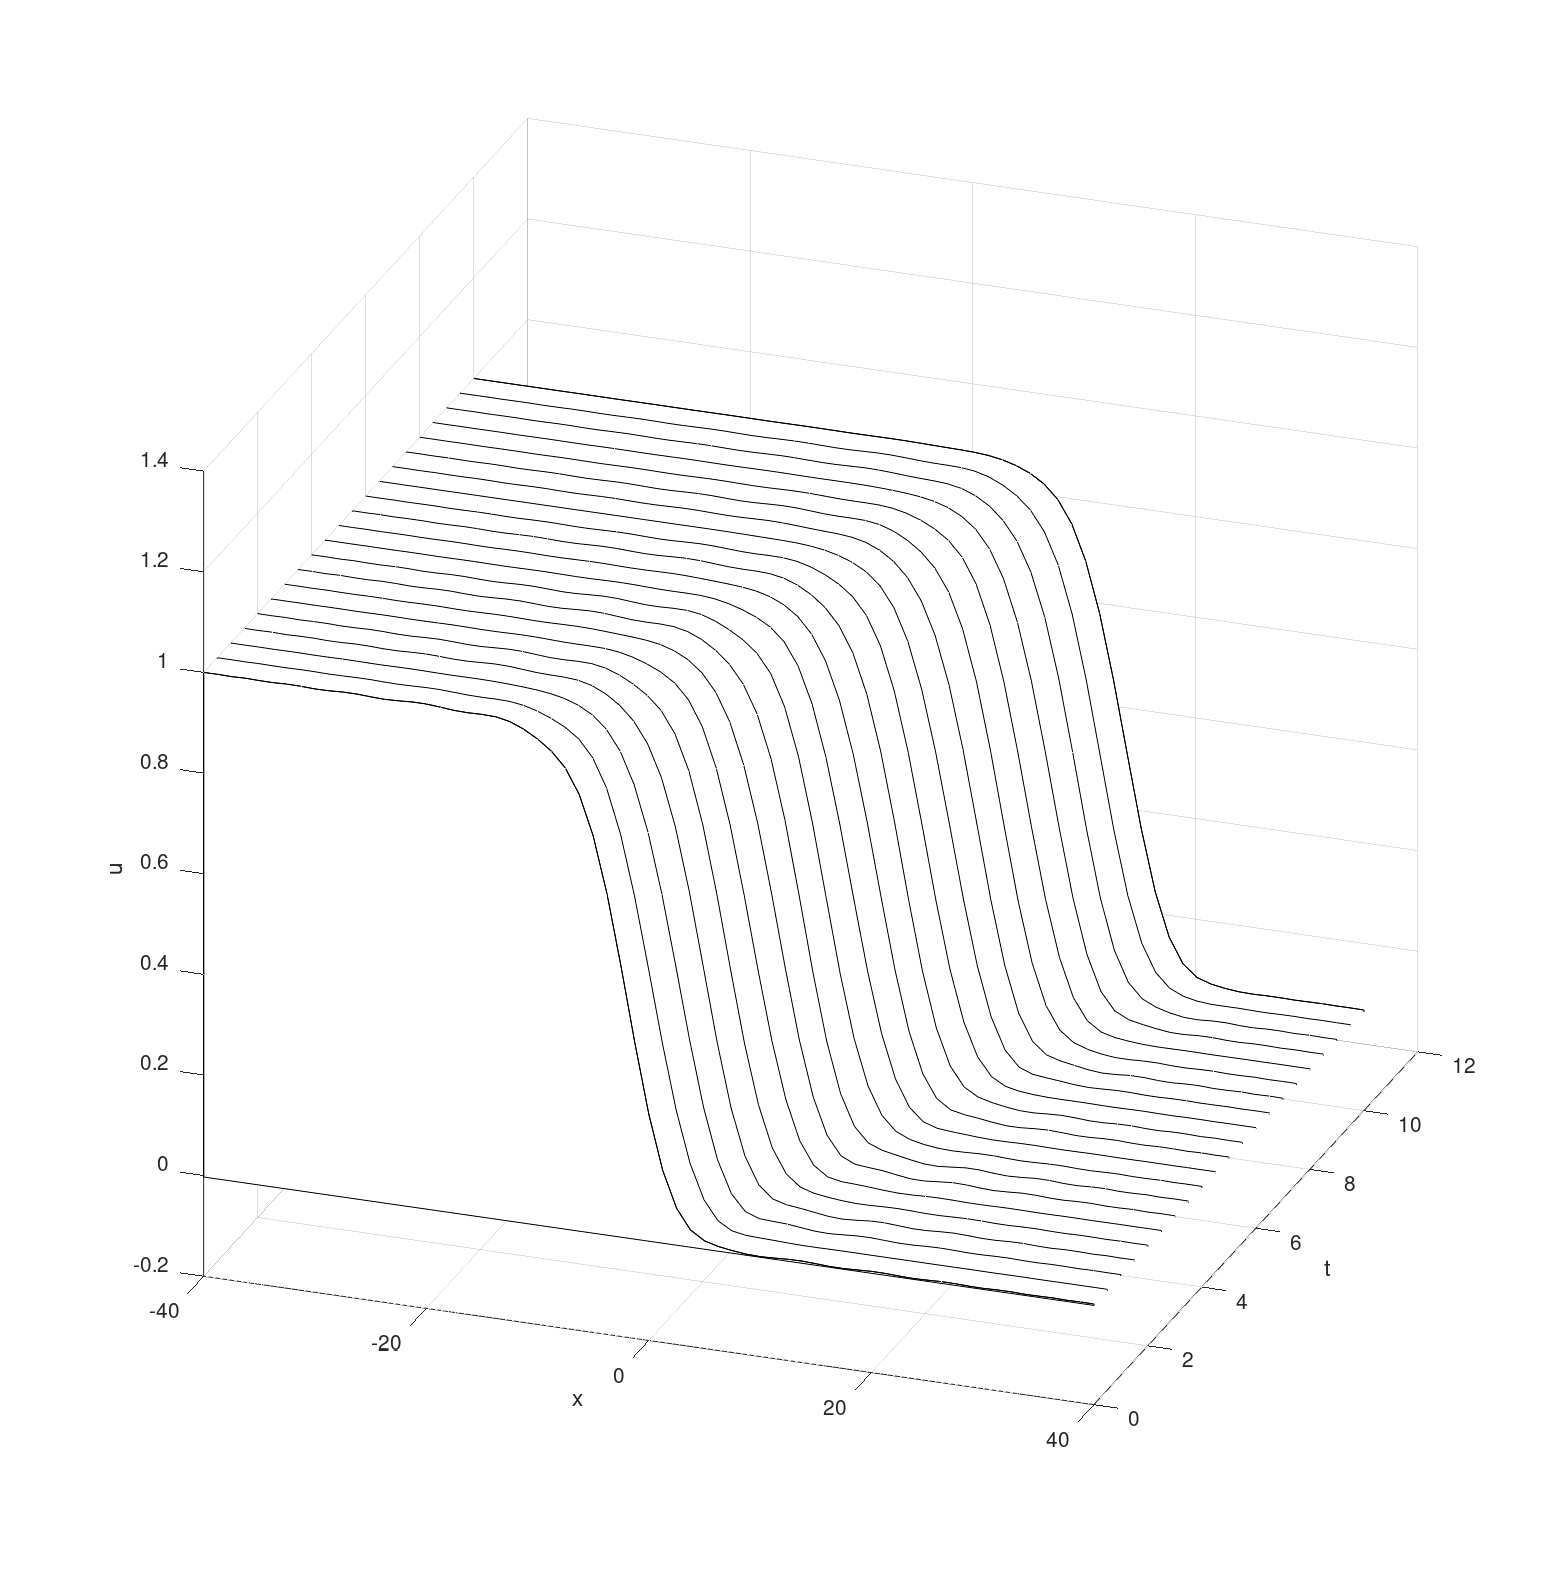
\includegraphics[width=\textwidth]{problem_2ii_L40.png}
        \end{subfigure}
        \hfill
        \begin{subfigure}[b]{0.49\textwidth}
            \centering
            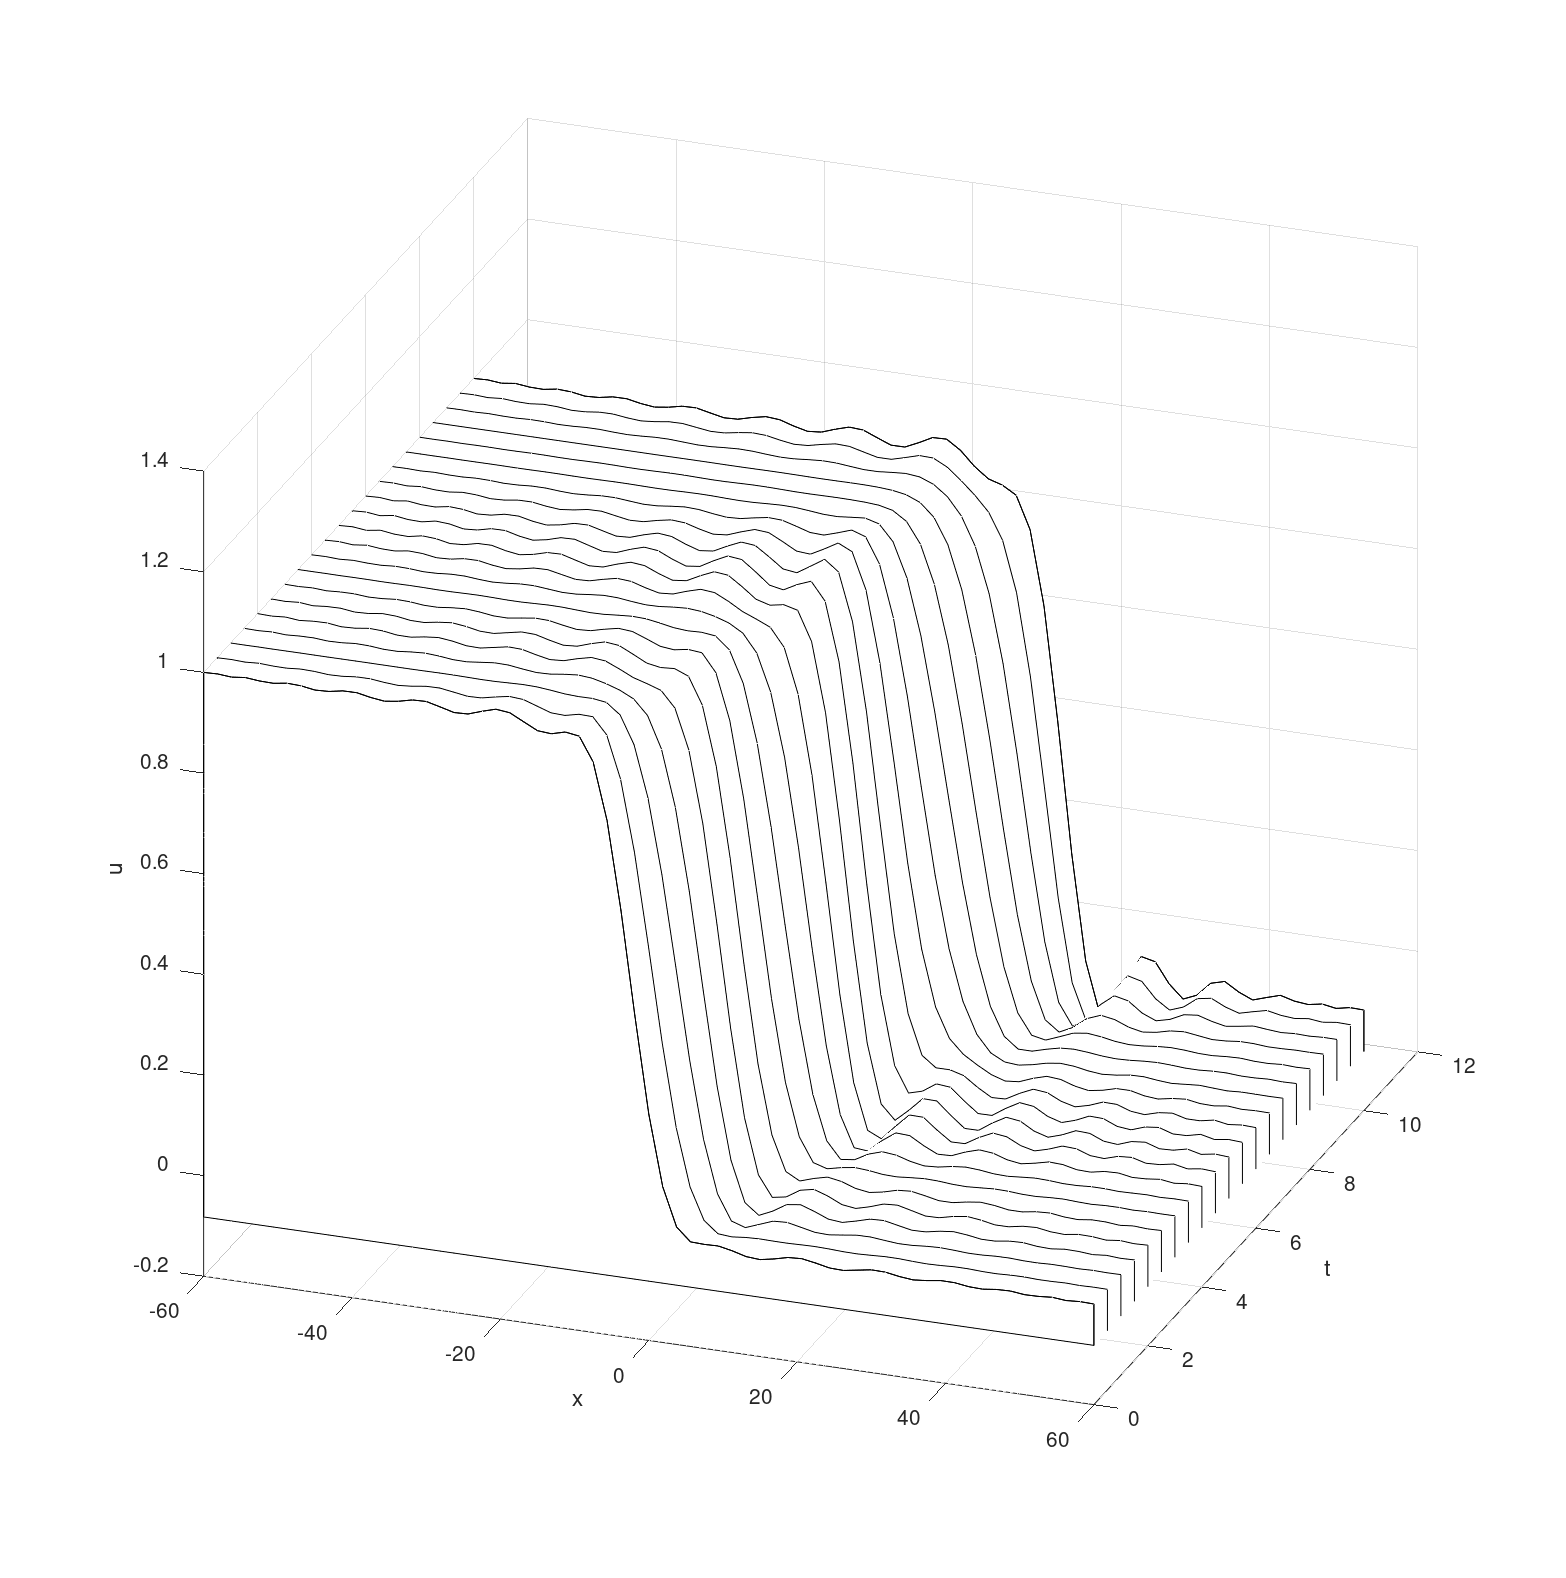
\includegraphics[width=\textwidth]{problem_2ii_L60.png}
        \end{subfigure}
        \caption{Fisher "front wave" solutions for $L = 40, 60$.}
        \label{fig:problem2ii_L30_L60}
    \end{figure*}
    \ \\
\end{solution}